\documentclass[capnocolon,titlechinese]{USTCthesis}
\usepackage{metalogo}
%\usepackage{floatrow}
\usepackage{verbatim}

% 设置图形文件的搜索路径
\graphicspath{{chapter/}{figures/}}
\begin{document}
%%%%%%%%%%%%%%%%%%%%%%%%%%%%%%
%% 封面部分
%%%%%%%%%%%%%%%%%%%%%%%%%%%%%%
  % 中文封面内容
  %如果使用\makeseparatetitle命令生成扉页,当中文标题过长时可以将多余的标题放在\titletail{}中
  \title{中国科学技术大学}
  \titletail{本科毕业论文模板示例文档}
  \entitle{An example article of the USTC-Thesis Template for Undergraduate Students}
  %全角空格可以正常输出
  \author{冯\ 盛}
  \enauthor{Sheng Feng}
  \department{物理学院\ 物理系}
  \No{PB06013016}
  \tutor{张三\ 教授}
  \entutor{Prof.San Zhang}
  \cntime{二〇一一年五月}
  \entime{May,2011}
  %生成封面(制本厂要求的格式)
  \makecover
  % 扉页形式
  %生成中英文合并的扉页
  \maketitle
  %生成中英文分开的扉页
  \makeseparatetitle

%%%%%%%%%%%%%%%%%%%%%%%%%%%%%%
%% 前言部分
%%%%%%%%%%%%%%%%%%%%%%%%%%%%%%
\frontmatter

  % 致谢
  
\begin{thankspage}
\noindent
{\bfseries From XPS:}\\
参考了以下内容:
ctex(Package), book.cls, cctbook.cls, article.cls, latex源代码, titlesec(doc)
, natbib(doc), caption(doc), fancyhdr(doc) 字号--pt对照表(From Web),
ustcthesis(博士论文测试版), bbs.ctex.org, www.wikipedia.org
感谢以上文档以及他们的维护者.

\noindent{\bfseries From heaven7:}\\
感谢XPS同学辛苦制作的模板。\\
参考内容见参考文献。

\noindent{\bfseries From ywg:}\\
对XPS同学的辛苦工作表示由衷的感谢!\\
感谢大家对本模板更新工作的支持!

\end{thankspage}

  % 目录

  \tableofcontents
  % 摘要
  
\begin{cnabstract}
本文是中国科学技术大学本科毕业论文的~\LaTeX{}~模板。本模板作者为XPS,本示例文档作者为heavenseven。2011年由ywg进行了部分更新

摘要部分由cnabstract和abstract两个环境组成,请用你自己的文字来代替这些文字。
\cnkeywords{中国科大,毕业论文,\LaTeX{}~模板}
\end{cnabstract}


\begin{abstract}
This article is a thesis template for undergraduate students of Univ.of Science and Technology of China.
The template is written by XPS, and heavenseven is the author of this article. Latest update is finished in 2011 by ywg. 

The abstract chapter consists of cnabstract environment and the abstract environment. Pls replace these words with your own to complete your abstract.
\keywords{Univ. of Science and Technology of China (USTC), Thesis, \LaTeX{} Template}
\end{abstract}



%%%%%%%%%%%%%%%%%%%%%%%%%%%%%%
%% 正文部分
%%%%%%%%%%%%%%%%%%%%%%%%%%%%%%
\mainmatter
  \chapter[本模板简单的使用说明]{本模板简单的使用说明\protect\footnote{本章由ywg添加}}
\section{模板基本信息}
\subsection{模板简介}
本模板是按照中国科学技术大学教务处规定制作的,适合于本科生毕业论文撰写的\LaTeX 模板,模板在ctexbook文档类的基础上进行了修改,添加了一些常用的宏包和命令。

\subsection{提出疑问及报告Bug}
如果您在使用过程中有疑问,遇到困难,可以在\href{http://bbs.ustc.edu.cn/cgi/bbsdoc?board=TeX}{瀚海星云\TeX{}讨论区}或者相关的\LaTeX 论坛(如\href{http://bbs.ctex.org}{CTEX 论坛})寻求帮助,但是请注意遵守论坛的各项规定。

如果使用过程中遇到Bug,请提交到\href{http://bbs.ustc.edu.cn/cgi/bbsdoc?board=TeX}{瀚海星云\TeX{}讨论区},或者提交到相应的\href{http://code.google.com/p/ustcthesis/issues/list}{Google UstcThesis Project(http://code.google.com/p/ustcthesis/issues/list)},请注明是本科论文模板的bug。

\subsection{如何得到本模板}
可以在\href{http://code.google.com/p/ustcthesis/downloads/list}{Google UstcThesis Project(http://code.google.com/p/ustcthesis/downloads/list)}下载到完整的模板文件(包括本说明文档)。

\section{模板基本设置}
使用本模板,您应首先具备基本的\LaTeX 知识,如果您刚刚接触\LaTeX,建议您先学习相关的用户文档或教程。

模板文件名为ustcthesis.cls。方便起见,将该文件放置在与论文主文件同一文件夹中即可。

模板提供一个文档类ustcthesis,使用\verb|\documentclass{ustcthesis}|来加载模板。

模板可以使用ctexbook文档类的相应选项,默认加载的是 12pt, a4paper, fancyhdr, fntef, twoside, opentight。需要注意的是默认加载 \emph{双面/章节从奇数页开始} 选项,如果需要\emph{单面} 选项,请使用:\begin{center}\verb|\documentclass[oneside,openany]{ustcthesis}|\end{center}

模板提供了两个新的文档选项 capnocolon 和 titlechinese,它们具体的效果如下:
\begin{description}
\item[capnocolon]{去掉图表标题序号中的“:”(\autoref{pic:capnocolon})}
\item[titlechinese]{章节标题使用中文格式(\autoref{pic:titlech})}
\end{description}

\begin{figure}
\centering
\subfigure[序号不带“:”]{\centering
  \framebox{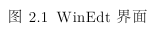
\includegraphics[scale=1]{figures/capnocolon.PNG}}}
\subfigure[序号带“:”]{\centering
  \framebox{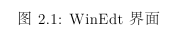
\includegraphics[scale=1]{figures/capcolon.PNG}}}
\figcaption{capnocolon选项效果及对比}
\label{pic:capnocolon}
\end{figure}

\begin{figure}
\centering
\subfigure[中文章节编号]{\centering
  \framebox{
\includegraphics[scale=0.52]{figures/titlech.PNG}}}
\subfigure[一般编号]{\centering
  \framebox{
\includegraphics[scale=0.505]{figures/titlearbic.PNG}}}
\figcaption{titlechinese选项效果及对比}
\label{pic:titlech}
\end{figure}

\section{模板提供的新环境}
模板提供了4个新环境\emph{abstract,cnabstract,thankspage,code}.分别是\emph{英文摘要,中文摘要,致谢,代码}环境,使用方法比较简单,这里不再赘述。

另外,针对数学等需求,定义若干新环境。模板提供的环境见\autoref{tab:env}
\begin{table}
\tabcaption{模板提供的新环境}
\label{tab:env}
\centering
\begin{tabular}{c|c||c|c}
\hline\hline
环境 & 含义 & 环境& 含义\\\hline\hline
abstract&英文摘要&cnabstract&中文摘要\\\hline
thankspage&致谢页&code&代码\\\hline
theorem &定理&lemma &引理  \\\hline
example &例&algorithm &算法  \\\hline
definition &定义  &axiom &公理  \\\hline
property &性质  &proposition &命题 \\\hline
corollary& 推论 &remark &注解  \\\hline
condition &条件  &conclusion &结论  \\\hline
assumption &假设  &prove &证明 \\\hline
proof&证明 &&\\ \hline\hline
\end{tabular}
\end{table}

需要注意的是,这里prove环境翻译为“证明”,事实上,其实prove环境不是用作theorem等类似环境配套证明的,prove环境是与theorem等环境同级别的环境。与theorem等环境相配套的证明环境是proof环境。使用时请注意下两个环境的差异:proof环境是没有编号的,是与theorem这类环境配合使用的;prove环境是有编号的,更多的是类似于证明题的题目。详细的差别见\autoref{pic:proofandprove}。

\begin{figure}
\centering
  \framebox{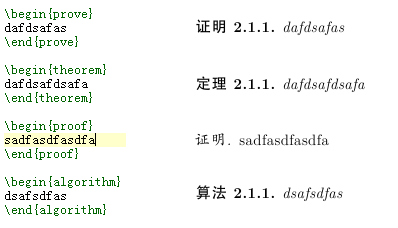
\includegraphics[scale=1]{figures/proofandprove.PNG}}
  \figcaption{proof、prove以及部分其他数学环境的差异}
  \label{pic:proofandprove}
\end{figure}


\section{模板提供的新命令}
主要的新命令如下:
\begin{description}
\item[\textbackslash figcaption\{\}]{效果是无论是否在图形环境中均生成图标题}
\item[\textbackslash tabcaption\{\}]{效果是无论是否在表格环境中均生成表标题}
\item[\textbackslash scite\{\}]{效果是得到如\scite{deng:01}这样的参考文献上标引用}
\item[\textbackslash chuhao]{改变字体大小为初号,类似的有\verb|\xiaoyihao|(小一号)直到\verb|\qihao|(七号)}
\item[\textbackslash makecover]{制作封面,供制本厂制作封面使用}
\item[\textbackslash maketitle]{制作扉页,中英文标题在一起}
\item[\textbackslash makeseparatetitle]{制作独立的中英文封面,中英文封面各一张\footnote{对于扉页格式,教务处没有规定,根据喜好二选一即可,或者自行发挥}}
\item[\textbackslash titletail\{\}]{中文标题过长的部分放在这个命令之中}
\item[\textbackslash tutor\{\}]{导师信息}
\item[\textbackslash entitle\{\}]{英文标题}
\item[\textbackslash entutor\{\}]{导师英文信息}
\item[\textbackslash cntime\{\}]{论文完成中文时间,自己填写}
\item[\textbackslash entime\{\}]{论文完成英文时间,自己填写}
\item[\textbackslash department\{\}]{院系中文名称}
\item[\textbackslash No\{\}]{学号}
\item[\textbackslash keywords\{\}]{英文关键字,在英文摘要环境中使用}
\item[\textbackslash cnkeywords\{\}]{中文关键字,在中文摘要环境中使用}
\item[\textbackslash L\{width\}]{表格环境中使用。对表格环境下p{width}命令进行加强,类似的还有C\{width\}和R\{width\}可以在指定宽度的同时指定对齐方式,三个命令分别表示左对齐、居中对齐、右对齐。注意大小写。(范例如下,效果如\autoref{tab:newcmd})}
\end{description}

\begin{minipage}{\textwidth}
\begin{verbatim}
\begin{table}
\tabcaption{几种命令效果对比的对比}
\label{tab:newcmd}
\centering
\begin{tabular}{c||l|c|r|p{2.5cm}|L{2.5cm}|C{2.5cm}|R{2.5cm}}
\hline
命令&l&c&r&p\{width\}&L\{width\}&C\{width\}&R\{width\}\\
\hline
效果&左齐&居中&右齐&定宽&左齐定宽&居中定宽&右齐定宽\\
\hline
\end{tabular}
\end{table}
\end{verbatim}

\tabcaption{几种命令效果对比的对比}
\label{tab:newcmd}
\centering
\begin{tabular}{c||l|c|r|p{2.5cm}|L{2.5cm}|C{2.5cm}|R{2.5cm}}
\hline
命令&l&c&r&p\{width\}&L\{width\}&C\{width\}&R\{width\}\\
\hline
效果&左齐&居中&右齐&定宽&左齐定宽&居中定宽&右齐定宽\\
\hline
\end{tabular}
\end{minipage}


\section{使用模板的一些注意事项}
把题目写在\verb|\title{}|中,只有题目过长的时候,再将过长的部分放在\verb|\titletail{}|中去(如\autoref{pic:title})。 

\begin{figure}
\centering
  \framebox{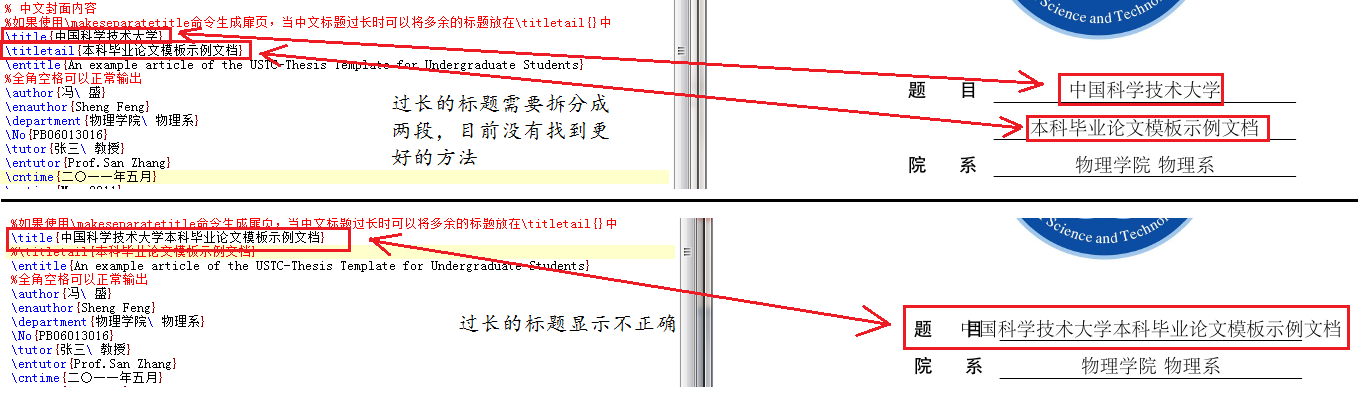
\includegraphics[scale=0.4]{figures/title}}
  \figcaption{过长的标题}
  \label{pic:title}
\end{figure}

比如:

对于短的题目——\\ \rule{4em}{0pt}\textbackslash title\{较短的题目\} 

对于较长的题目——\\\rule{4em}{0pt}\textbackslash title\{较长的题目的前一部分\} 
\\\rule{4em}{0pt}\textbackslash titletail\{较长的题目的后一部分\}

公式、章节、图和表格等(不包括脚注和参考文献)的交叉引用可以使用\verb|\autoref{label}|来得到正确的引用。例如使用\verb|\autoref{some_pic}|可以得到“图 X”的引用,使用\verb|\autoref{some_table}|可以得到“表 X”的引用。

建议使用\verb|\figcaption{}|命令得到所有图形的标题,表格也是。这样无论是否在图形环境中均能够得到正确的带图/表编号的标题,而在图形环境之外使用\verb|\caption{}|命令会报错。

封面是按照制本厂的要求制作的,其中行宽和行高都是固定的,中文标题最多占两行,英文标题最多占三行。如果您的题目超过了这个限制,请缩减题目长度,不要擅自修改模板中的相关配置参数。


  
\chapter{绪论}
\label{chap:introduction}

中国科学技术大学,中国科学技术大学,中国科学技术大学,中国科学技术大学,中国科学技术大学,中国科学技术大学
中国科学技术大学,中国科学技术大学,中国科学技术大学


中国科学技术大学

\section{系统要求}



\section{下载与安装}


\href{http://code.google.com/p/ustcthesis}{http://code.google.com/p/ustcthesis}




\section{问题反馈}

用户在使用中遇到问题或者需要增加某种功能,请到\href{http://bbs.ustc.edu.cn/cgi/go?cgi=bbsdoc&board=TeX}{瀚海星云bbs,Tex版}反映。


欢迎大家反馈自己的使用情况,使我们可以不断改进宏包。

\section{为人民服务}


我们的共产党和共产党所领导的八路军、新四军,是革命的队伍。我们这个队伍完全是为着解放人民的,是彻底地为人民的利益工作的。张思德同志就是我们这个队伍中的一个同志。

人总是要死的,但死的意义有不同。中国古时候有个文学家叫做司马迁的说过:人固有一死,或重于泰山,或轻于鸿毛。为人民利益而死,就比泰山还重;替法西斯卖力,替剥削人民和压迫人民的人去死,就比鸿毛还轻。张思德同志是为人民利益而死的,他的死是比泰山还要重的。因为我们是为人民服务的,所以,我们如果有缺点,就不怕别人批评指出。不管是什么人,谁向我们指出都行。只要你说得对,我们就改正。你说的办法对人民有好处,我们就照你的办。“精兵简政”这一条意见,就是党外人士李鼎铭⑶先生提出来的;他提得好,对人民有好处,我们就采用了。只要我们为人民的利益坚持好的,为人民的利益改正错的,我们这个队伍就一定会兴旺起来。

我们都是来自五湖四海,为了一个共同的革命目标,走到一起来了。我们还要和全国大多数人民走这一条路。我们今天已经领导着有九千一百万人口的根据地,但是还不够,还要更大些,才能取得全民族的解放。我们的同志在困难的时候,要看到成绩,要看到光明,要提高我们的勇气。中国人民正在受难,我们有责任解救他们,我们要努力奋斗。要奋斗就会有牺牲,死人的事是经常发生的。但是我们想到人民的利益,想到大多数人民的痛苦,我们为人民而死,就是死得其所。不过,我们应当尽量地减少那些不必要的牺牲。我们的干部要关心每一个战士,一切革命队伍的人都要互相关心,互相爱护,互相帮助。

今后我们的队伍里,不管死了谁,不管是炊事员,是战士,只要他是做过一些有益的工作的,我们都要给他送葬,开追悼会。这要成为一个制度。这个方法也要介绍到老百姓那里去。村上的人死了,开个追悼会。用这样的方法,寄托我们的哀思,使整个人民团结起来。
  \chapter{正文写作}
\label{c:main}
本章中介绍了一些\LaTeX 不得不说的基础知识,包括\LaTeX 语句的基本概念,\LaTeX 中的特殊字符,章节命令,空格、分行和段落等等。



\section{\LaTeX 语句}
\LaTeX 语句主要有命令、数据和注释组成。命令有控制词和控制符两种,其中控制词以右斜杠\verb|\|开始,以非字母字符结束(如\verb|\textbackslash|);控制符以\textbackslash 开始,紧跟着一个非字母、数字的字符(如\verb|\;|)。注释以\%开始,每行自\%之后的内容都不会被编译。

命令可能会有一些参数,如
\begin{code}
        \includegraphics[width=10cm]{1.jpg}
\end{code}
其中中括号括起来的是可选参数,当省略时,\LaTeX{}会根据默认值来选择;大括号内的是不可省略的参数。这个命令的含义见第\ref{chap:fig}章。

\section{\LaTeX 中的特殊字符}
\subsection{空格与回车}
在\LaTeX 中,连续的空格被认为是一个空格。行首的空格通常被忽略。按下回车产生的断行也被认为是空格。\par
而当为了美观需要,不得不强行插入空格时,有很多选择,这里给出其中的一部分:
\begin{itemize}
\item{}\verb|~|,产生不可断行的半个空格;
\item{}\verb|\ |,即\verb|\|之后再加一个空格,产生1/3个字母m宽度空格;
\item{}\verb|\hspace{1cm}|,其中1cm可以随便替换,需要加长度单位,如em,pt等;
\item{}\verb|\quad|,一个字母m的宽度;
\item{}\verb|\qquad|,两个字母m的宽度;
\end{itemize}

一个回车会得到一个空格,而两个回车会得到一个空行,空行代表开始一个新段落。连续的空行被当作是一个空行。

\subsection{引号}
左右引号分别用不同的字符\verb|`|(数字1左边的键)和\verb|'|(通常所用的单引号)表示。双引号则是连续两个左引号+连续两个右引号。
\begin{figure}[h]
\centering
\fbox{\begin{minipage}[h]{0.4\textwidth}
我听见韩麦尔先生对我说:``唉,总要把学习拖到明天,这正是阿尔萨斯人最大的不幸。现在那些家伙就有理 由对我们说了:`怎么?你们还自己说是法国人呢,你们连自己的语言都不会说,不会写!……'不过,可怜的小弗郎 士,也并不是你一个人的过错。''
\end{minipage}}
\hspace{0.1\textwidth}
\begin{minipage}[h]{0.4\textwidth}
\centering
\begin{code}
我听见韩麦尔先生对我说:``唉,总要把学习拖到明天,这正是阿尔萨斯人最大的不幸。现在那些家伙就有理 由对我们说了:`怎么?你们还自己说是法国人呢,你们连自己的语言都不会说,不会写!……'不过,可怜的小弗郎 士,也并不是你一个人的过错。''
\end{code}
\end{minipage}
\caption{引号}
\label{f:quote}
\end{figure}

\subsection{控制字符}
以下这些是\LaTeX 中的控制字符:
\begin{code}
              #  $  %  ^  &  _  {  }  ~  \
\end{code}
它们被用作控制符,因而不能直接输入。要输入这些字符,分别可以用以下命令:
\begin{code}
        \#   \$  \%   \^{}  \&  \_  \{  \}  \~{}  \textbackslash
\end{code}
可以看到,一般来说,在这些字符前加上右斜杠\verb|\|,就可以正常输出。\verb|\\|除外,这是一个换行命令(见下一节)。\par

\subsection{横线}
一个短横线\verb|-|代表连字符,两个短横线\verb|--|会产生一个用于数字范围的短破折号,三个短横线\verb|---|产生普通的破折号。而代表负数的负号则应该是\verb|$-$|。

\section{控制字体样式}
大部分时候,\LaTeX{}会自动控制字样。当为了强调某些文字,需要改变字体时,以下有一些例子:
\begin{center}
\begin{tabular}{ll@\qquad ll}
\whline
\verb|\textrm{...}|& \textrm{roman}& \verb|\textbf{...}|& \textbf{bold face}\\
\verb|\textsf{...}| &\textsf{sans serif}& \verb|\textit{...} |&\textit{italic}\\
\verb|\texttt{...}|& \texttt{typewriter} &\verb|\textsl{...}|& \textsl{slanted}\\
\verb|\emph{...}|& \emph{emphasized}& \verb|\underline{...}|& \underline{underline}\\
\whline
\end{tabular}
\end{center}

表中列出了大部分常用的文字样式选择命令,使用时将需要改变字样的文字放在命令后的大括号中作为参数即可。

\section{改变字体大小}
ustcthesis模板中提供了字号选择命令:
\begin{code}
        \chuhao,\xiaochuhao,\yihao,\erhao,\xiaoerhao,...\qihao
\end{code}
一个简单的例子:
\begin{figure}[h]
\centering
\fbox{\begin{minipage}[h]{0.4\textwidth}
{\chuhao 初号}\\
{\sihao 四号文字}\\
{\qihao 七号文字}
\end{minipage}}
\hspace{0.1\textwidth}
\begin{minipage}[h]{0.4\textwidth}
\centering
\begin{code}
{\chuhao 初号}\\
{\sihao 四号文字}\\
{\qihao 七号文字}
\end{code}
\end{minipage}
\caption{字号选择}
\label{f:size}
\end{figure}

如例子中的那样,对于一段需要改变字号的文字,应当用大括号将其包围起来,将字号选择命令置于大括号开头。这样做可以防止字号选择命令影响之后的文字。

正文中默认使用的字号是小四号。

\section{控制空格,分行,分段,分页,章节}
\begin{description}
\item{\textbf{分行}}
这里我们说的是段内分行。在\LaTeX 中,普通的回车会被视为空格,而分行的命令则是\verb|\\|。分行与分段的区别在于下一行的段首不会缩进,并且
这两行之间的间距还是普通行间距,比段间距要小。
\item{\textbf{分段}}
一个空行意味着一段的结束和下一段的开始。也可以使用分段符:\verb|\par|。
\item{\textbf{分页}}
使用\verb|\newpage|命令强制分页。
\item{\textbf{章节}}
\LaTeX 使用章节类命令控制文章结构。章节类命令可以自动生成对应的格式,并且会自动插入目录中。\par
对于本科毕业论文,从大到小的章节依次为:\\
\begin{minipage}{0.8\textwidth}
\begin{code}
    \chapter,\section,\subsection,\subsubsection
\end{code}
\end{minipage}\\
章节命令的参数是该章节的名字。
\end{description}

\section{环境}
环境命令(environment)是一类特殊的\LaTeX{}命令。通常,一个环境命令定义了环境内部的字体、对齐和缩进方式、自动编号等信息,用于方便用户输入公式、注释、引文等。一个环境命令如下:
\begin{code}
            上文
            \begin{环境名}
                ...
                环境内的文字
                ...
            \end{环境名}
            下文
\end{code}

几个常用的环境有:
\begin{itemize}
\item center:居中
\item quote:引文
\item verbatim:原文照排,即不经过处理,直接按原样输出。
\item enumerate:自动编号的有序列表
\item itemize:枚举,带有项目符号的无序列表
\end{itemize}

\begin{example}{quote环境}\\
quote环境会自动设置缩进量和上下行距,如下图。
\begin{figure}[h]
\centering
\fbox{\begin{minipage}[h]{0.4\textwidth}
唐伯虎曾经写道:
\begin{quote}
别人笑我太疯癫,\\我笑他人看不穿。
\end{quote}
引自《桃花庵》。
\end{minipage}}
\hspace{0.1\textwidth}
\begin{minipage}[h]{0.4\textwidth}
\centering
\begin{code}
唐伯虎曾经写道:
\begin{quote}
别人笑我太疯癫,\\我笑他人看不穿。
\end{quote}
引自《桃花庵》。
\end{code}
\end{minipage}
\end{figure}
\end{example}

在itemize和enumerate环境中用item命令表示列举项。两者可以互相嵌套,如图\ref{f:item}。
\begin{figure}[!h]
\centering
\fbox{\begin{minipage}[h]{0.4\textwidth}
\begin{itemize}
\item fruit
\begin{itemize}
\item apple
\item strawberry
\end{itemize}
\item drinks
\begin{enumerate}
\item coffee
\item tea
\end{enumerate}
\item chocolate
\end{itemize}
\end{minipage}}
\hspace{0.1\textwidth}
\begin{minipage}[h]{0.4\textwidth}
\centering
\begin{code}
\begin{itemize}
    \item fruit
    \begin{itemize}
        \item apple
        \item strawberry
    \end{itemize}
    \item drinks
    \begin{enumerate}
        \item coffee
        \item tea
    \end{enumerate}
    \item chocolate
\end{itemize}
\end{code}
\end{minipage}
\caption{itemize和enumerate}
\label{f:item}
\end{figure}

关于其他数学环境以及公式的输入,请参阅第\ref{chap:math}章的相关内容。 
   
\chapter{数学公式}
\label{chap:math}
\begin{equation}
\begin{split}
\mbox{Pr}\{S_i=0\}=\frac{a_i}{b_i+a_i} \\
\mbox{Pr}\{S_i=1\}=\frac{b_i}{b_i+a_i} \label{1}
\end{split}
\end{equation}\cite{lshort-cn}



\begin{table}[htbp]
\centering
\caption{基于因子分析的失配补偿结果}\label{tab:jfa-gmm-ubm}
\begin{tabular}{cccccc}
    \toprule
    &\multirow{2}{*}{\#Mix}&\multicolumn{2}{c}{No-norm}
    &\multicolumn{2}{c}{Tnorm}\\
    \cline{3-4} \cline{5-6}
		&		& EER(\%) 	& MinDCF & EER(\%) 	& MinDCF\\
    \midrule
	\multirow{3}{*}{GMM-UBM}
    &256 		& 12.43 	& 0.0647	& 12.85    & 0.0580\\
    &512 		& 10.02 	& 0.0464	& 8.88 	   & 0.0370\\
    &1024 		& 9.97 	    & 0.0457	& 8.72 	   & 0.0372\\
    \midrule
	\multirow{3}{*}{Factor Analysis}
    &256 		& 8.09 	& 0.0331 	& 7.39 	& 0.0319\\
    &512 		& 7.08 	& 0.0305 	& 6.53 	& 0.0292\\
    &1024 		& 6.83 	& 0.0295 	& \textbf{6.29} 	& \textbf{0.0279}\\
 \bottomrule
\end{tabular}
\end{table}



\IncMargin{1em}
\begin{algorithm}
\SetKwData{Left}{left}\SetKwData{This}{this}\SetKwData{Up}{up}
\SetKwFunction{Union}{Union}\SetKwFunction{FindCompress}{FindCompress}
\SetKwInOut{Input}{input}\SetKwInOut{Output}{output}
\Input{$O_t,UBM,U$}
\Output{$x,y$}
\BlankLine
\emph{$y\leftarrow 0;$$x_h\leftarrow 0;$$h=1,...,H$ }\;
\For{$i=1$ \KwTo Number of E-M iterations}{
\emph{E Step}:\\
\For{$h=1$ \KwTo $H$}{\label{forins}
对于每一条语音段,计算其EM统计量(零阶统计量$N_h$,一阶统计量$S_{X,h}$\;
}
计算每一个人所有语音段的零阶统计量$N$\\
计算每一个人所有语音段的一阶统计量$S$\\
\emph{M Step}:\\
\For{$j=1$ \KwTo Number of Gauss-Seidel iterations}{
\For{$h=1$ \KwTo $H$}{\label{forins}
估计每一语音段$h$的失配因子$x_h$
}
估计模型的话者因子$y$
}
}
\Return{$\mu = m+Dy$}
\caption{disjoint decomposition}\label{algo_disjdecomp}
\end{algorithm}\DecMargin{1em}
   
\chapter{图形}
\label{chap:fig}


\section{浮动图形}

\XeLaTeX 支持jpg和eps格式的图片。我们所用的编译方法支持jpg和eps等格式的图片。如果你已经有一篇word文档,
想把其中的图全部导出,那么可以将它另存为html文件,这时会在同目录下找到一个文件夹,里面是所有用到的图片。

将插图放在figures文件夹中,想要引用的地方使用类似这样的命令插入图形文件:
\begin{code}
\begin{figure}[!ht]
 \centering
 
\includegraphics[width=0.2\textwidth]{ustc_logo_new.eps}
 \caption{中国科学技术大学校徽(在页面中间)}
 \label{fig:ustc1}
\end{figure}
\end{code}
结果如下:
\begin{figure}[!ht]
 \centering
 
\includegraphics[width=0.2\textwidth]{ustc_logo_new.eps}
 \caption{中国科学技术大学校徽(在页面中间)}
 \label{fig:ustc1}
\end{figure}

在上面这段命令中,可选参数[!ht]代表插图的位置。其中!让\LaTeX{}忽略审美标准,试图用最严格的标准来放置浮动图形;h(ere)代表有限放在此处;t(op)代表如果此处放不下,那么放在下一页页首。

width=0.2\textbackslash{}textwidth代表图形的宽度是文字宽度的0.2倍,你也可以使用其他长度单位,如12cm,4.5in等等。

caption命令的参数代表图的名称,或者说注解。label的参数用于交叉引用,见下节。


\section{交叉引用}
通过使用交叉引用功能,我们可以定位那些\LaTeX{}自动编号的内容,比如浮动图形、表格、章节等等。其中,label和ref的参数是引用的名字,可以随意,但须保持一致。
\begin{figure}[ht]
\centering
\fbox{\begin{minipage}[h]{0.4\textwidth}
引用图\ref{fig:ustc1}\\
引用第\ref{chap:introduction}章
\end{minipage}}
\hspace{0.1\textwidth}
\begin{minipage}[h]{0.4\textwidth}
\centering
\begin{code}
引用图\ref{fig:ustc1}\\
引用第\ref{chap:introduction}章
\end{code}
\end{minipage}
\caption{交叉引用示例}
\end{figure}


\section{并列的子图}
使用subfigure命令,一个例子:
\begin{figure}[!hbt]
\centering
\subfigure[sf 1]{

\includegraphics[width=0.2\textwidth]{ustc_logo_new.eps}\label{f:1}}
\subfigure[sf 2]{

\includegraphics[width=0.2\textwidth]{ustc_logo_new.eps}\label{f:2}}
\subfigure[sf 3]{

\includegraphics[width=0.2\textwidth]{ustc_logo_new.eps}\label{f:3}}
\subfigure[sf 4]{

\includegraphics[width=0.2\textwidth]{ustc_logo_new.eps}\label{f:4}}
\caption{\label{f:s}subfigure使用示例。}
\end{figure}
\begin{code}
\begin{figure}[!hbt]
\centering
\subfigure[sf 1]{

\includegraphics[width=0.2\textwidth]{ustc_logo_new.eps}\label{f:1}}
\subfigure[sf 2]{

\includegraphics[width=0.2\textwidth]{ustc_logo_new.eps}\label{f:2}}
\subfigure[sf 3]{

\includegraphics[width=0.2\textwidth]{ustc_logo_new.eps}\label{f:3}}
\subfigure[sf 4]{

\includegraphics[width=0.2\textwidth]{ustc_logo_new.eps}\label{f:4}}
\caption{\label{f:s}subfigure使用示例。}
\end{figure}
\end{code}

分两行放:
\begin{figure}[!hbt]
\centering
\subfigure[sf 1]{

\includegraphics[width=0.2\textwidth]{ustc_logo_new.eps}\label{f:1}}
\subfigure[sf 2]{

\includegraphics[width=0.2\textwidth]{ustc_logo_new.eps}\label{f:2}}\\
\subfigure[sf 3]{

\includegraphics[width=0.2\textwidth]{ustc_logo_new.eps}\label{f:3}}
\subfigure[sf 4]{

\includegraphics[width=0.2\textwidth]{ustc_logo_new.eps}\label{f:4}}
\caption{\label{f:s}subfigure使用示例。}
\end{figure}
\begin{code}
\begin{figure}[!hbt]
\centering
\subfigure[f 1]{

\includegraphics[width=0.2\textwidth]{ustc_logo_new.eps}\label{f:1}}
\subfigure[f 2]{

\includegraphics[width=0.2\textwidth]{ustc_logo_new.eps}\label{f:2}}\\
\subfigure[f 3]{

\includegraphics[width=0.2\textwidth]{ustc_logo_new.eps}\label{f:3}}
\subfigure[f 4]{

\includegraphics[width=0.2\textwidth]{ustc_logo_new.eps}\label{f:4}}
\caption{\label{f:l}分行的字图使用示例。}
\end{figure}
\end{code}
   
\chapter{表格}
\label{chap:tab}
标准三线表:
\begin{table}[!ht]
\label{tab:table3}
\caption{三线表格示例}
\centering
\begin{tabular}{c c c c}
\whline 一列 & 两列 & 三列 & 四列  \\\hline
1 & 2 &3 &4 \\2 & 3 &4 &5 \\3 & 4 &5 &6 \\
\whline
\end{tabular}
\end{table}
\begin{code}
    \begin{table}[!ht]
    \label{tab:table3}
    \caption{三线表格示例}
    \centering
    \begin{tabular}{c c c c}
        \whline 一列 & 两列 & 三列 & 四列  \\\whline
        1 & 2 &3 &4 \\2 & 3 &4 &5 \\3 & 4 &5 &6 \\
        \whline
    \end{tabular}
    \end{table}
\end{code}

与figure一样,table环境也是浮动体,常用!ht来表明位置。caption、label的意义都与figure环境相同。

而画表格的tabular环境则与array环境几乎相同,只是在每行之间可以用\textbackslash{}hline和\textbackslash{}hline这些命令来画横线。c代表一个居中对齐的列,l代表靠左对齐,r代表靠右对齐。
有竖线的例子:
\begin{table}[!ht]
\label{tab:table2}
\caption{表格示例2}
\centering
\begin{tabular}{ Ic|c|c|cI}
\whline 一列 & 两列 & 三列 & 四列  \\\hline
1 & 2 &3 &4 \\\hline 2 & 3 &4 &5 \\\hline3 & 4 &5 &6 \\
\whline
\end{tabular}
\end{table}
\begin{code}
    \begin{table}[!ht]
    \label{tab:table2}
    \caption{表格示例2}
    \centering
    \begin{tabular}{ Ic|c|c|cI}
        \whline 一列 & 两列 & 三列 & 四列  \\\hline
        1 & 2 &3 &4 \\\hline 2 & 3 &4 &5 \\\hline3 & 4 &5 &6 \\
        \whline
    \end{tabular}
    \end{table}
\end{code}

即竖线是|,粗竖线是大写字母I,横线是\textbackslash hline,粗横线是\textbackslash whline。

  \chapter{参考文献的使用}
\label{c:bib}

本模板使用bibtex来管理参考文献。在BibTeX中,典型的参考文献信息如下:
\begin{code}
    @book{deng:01,
        author =       {{邓建松,~彭冉冉,~陈长松}},
        title =        {\LaTeXe{}~科技排版指南},
        publisher =    {科学出版社,~书号:~7-03-009239-2/TP.1516},
        year =         {2001},
        address =      {北京},
    }
\end{code}

其中,第一行的\@book指明了文献的类别;deng:01是引用时的标号,可以随意。在大括号之内则指明了参考文献信息,大家可以望文生义。在正文中参考文献的方法如下:
\begin{figure}[h]
\centering
\fbox{\begin{minipage}[t]{0.4\textwidth}
引用示例\cite{deng:01}
\end{minipage}}
\hspace{0.1\textwidth}
\begin{minipage}[t]{0.4\textwidth}
\centering
\begin{code}
引用示例\cite{deng:01}
\end{code}
\end{minipage}
\end{figure}

引用时还有许多选择,如下:\\
\begin{center}
\begin{tabular}{ll}
\whline
\verb|\citet{deng:01}|  &   \citet{deng:01}\\
\verb|\citep[p.~99]{deng:01}|&  \citep[p.~99]{deng:01}\\
\verb|\citep[e.g.][]{deng:01}|& \citep[e.g.][]{deng:01}\\
\verb|\citep[e.g.][p.~99]{deng:01}| &\citep[e.g.][p.~99]{deng:01}\\
\verb|\citeauthor{deng:01}|& \citeauthor{deng:01}\\
\verb|\citeyear{deng:01}|&\citeyear{deng:01}\\
\whline
\end{tabular}
\end{center} 
  
\chapter{常见问题}
\label{chap:faq}

\newtheoremstyle{question}% name
  {}%      Space above, empty = `usual value'
  {}%      Space below
  {\tt}% Body font
  {}%         Indent amount (empty = no indent, \parindent = para indent)
  {\bfseries}% Thm head font
  {.}%        Punctuation after thm head
  {10pt}% Space after thm head: \newline = linebreak
  {}%         Thm head spec

\newtheoremstyle{answer}% name
  {}%      Space above, empty = `usual value'
  {}%      Space below
  {\rm}% Body font
  {}%         Indent amount (empty = no indent, \parindent = para indent)
  {\bfseries}% Thm head font
  {.}%        Punctuation after thm head
  {10pt}% Space after thm head: \newline = linebreak
  {}%         Thm head spec

\theoremstyle{question}
 \newtheorem{FAQ}{问题~}
\theoremstyle{answer}
 \newtheorem{ANS}{回答~}

\section{表格}

\begin{FAQ}
页眉里论文题目和各章标题中的字母均为大写,不能实现大小写的区别,而我写的论文需要在页眉中出现的标题中区分英文字母的大小写比如:YBaCuO而不是YBACUO。
\end{FAQ}

\begin{ANS}
在 CASthesis.cfg 文件中加上
\begin{verbatim}
\renewcommand\title[2][\CAST@value@title]{%
  \def\CAST@value@title{#2}
  \def\CAST@value@titlemark{#1}}
\def\chaptermark#1{\markboth {{\ifnum \c@secnumdepth>\m@ne
  \if@mainmatter\CTEXthechapter \quad\fi
  \fi #1}}{}}%
\def\sectionmark#1{\markright{{\ifnum \c@secnumdepth >\z@
  \CTEXthesection \quad \fi #1}}}
\end{verbatim}
\end{ANS}


\section{脚注}

\begin{FAQ}
如果在章节标题中加入注脚,则不仅会出现在本章首页的页脚,也会出现在目录的页脚,不知是否能够让其不要出现在目录的页脚中。
\end{FAQ}

\begin{ANS}
可以使用如下的命令来定义章节的标题
\begin{verbatim}
\chapter[出现在目录和页眉的标题]{出现在正文的标题\footnote{这个不会出现在目录中。}}
\end{verbatim}
section、~subsection 等命令也有类似的用法。
\end{ANS}


%%%%%%%%%%%%%%%%%%%%%%%%%%%%%%
%% 附件部分
%%%%%%%%%%%%%%%%%%%%%%%%%%%%%%
%\backmatter

  % 参考文献
  % 使用 BibTeX
  \phantomsection
  \addcontentsline{toc}{chapter}{参考文献}
  \bibliography{bib/tex}
  \nocite{*} % for every item


  % 附录
  \begin{appendix}
    
\chapter{附录}
\label{chap:appendix}

附录是作为说明书(论文)的补充部分,并不是必需的。
\begin{enumerate}
\item{}下列内容可以作为附录编于说明书(论文)之后:
\begin{enumerate} \item{}为了说明书(论文)的完整,但编入正文又损于正文的处理和逻辑性,这一类材料包括比正文更为详细的信息研究方法和技术的途述,对于了解正文内容具有重要的补充意义;
\item{}由于篇幅过大或取材于复制品而不便编入正文的材料;
\item{}某些重要的原始数据、数学推导、计算程序、注释、框图、统计表、打印机输出样片、结构图等。
\end{enumerate}
\item{}
附录中的有关格式\\
  说明书(论文)的附录依次为“附录A”、“附录B”、“附录C”等编号。如果只有一个附录,也应编为“附录A”。\\
  附录中的图、表、公式的命名方法也采用上面提到的图、表、公式命名方法,只不过将章的序号换成附录的序号。
\end{enumerate}

  \end{appendix}



\end{document}
